% $Header: /cvsroot/latex-beamer/latex-beamer/solutions/conference-talks/conference-ornate-20min.en.tex,v 1.6 2004/10/07 20:53:08 tantau Exp $

\documentclass{beamer}
%\documentclass[handout]{beamer}
%\usepackage{pgfpages}
%\pgfpagesuselayout{2 on 1}[a4paper,border shrink=5mm]

% This file is a solution template for:

% - Talk at a conference/colloquium.
% - Talk length is about 20min.
% - Style is ornate.



% Copyright 2004 by Till Tantau <tantau@users.sourceforge.net>.
%
% In principle, this file can be redistributed and/or modified under
% the terms of the GNU Public License, version 2.
%
% However, this file is supposed to be a template to be modified
% for your own needs. For this reason, if you use this file as a
% template and not specifically distribute it as part of a another
% package/program, I grant the extra permission to freely copy and
% modify this file as you see fit and even to delete this copyright
% notice.


\mode<presentation>
{
%  \usetheme{Warsaw}
%  \usetheme{Boadilla}
%  \usetheme{Goettingen}
%  \usetheme{Hannover}
%  \usetheme{Madrid}
%  \usetheme{Marburg}
%  \usetheme{Montpellier}
%  \usetheme{Pittsburgh}
  \usetheme{Hawke}
  % or ...

  \setbeamercovered{transparent}
  % or whatever (possibly just delete it)
}


\usepackage[english]{babel}
% or whatever

\usepackage[latin1]{inputenc}
% or whatever

\usepackage{times}
\usepackage[T1]{fontenc}
% Or whatever. Note that the encoding and the font should match. If T1
% does not look nice, try deleting the line with the fontenc.

\usepackage{multimedia}


%%%%%%
% My Commands
%%%%%%

\newcommand{\ml}{{\sc matlab}}
\newcommand{\bb}{{\boldsymbol{b}}}
\newcommand{\bx}{{\boldsymbol{x}}}
\newcommand{\by}{{\boldsymbol{y}}}
\newcommand{\bfm}[1]{{\boldsymbol{#1}}}
\newcommand{\pda}[2]{\frac{\partial{#1}}{\partial{#2}}}


%%%%

\title[Lecture 21] % (optional, use only with long paper titles)
{Lecture 21 - Function basis methods for Boundary Value Problems}

% \subtitle
% {Include Only If Paper Has a Subtitle}

\author[I. Hawke] % (optional, use only with lots of authors)
{I.~Hawke}
% - Give the names in the same order as the appear in the paper.
% - Use the \inst{?} command only if the authors have different
%   affiliation.

\institute[University of Southampton] % (optional, but mostly needed)
{
%  \inst{1}%
  School of Mathematics, \\
  University of Southampton, UK
}
% - Use the \inst command only if there are several affiliations.
% - Keep it simple, no one is interested in your street address.

\date[Semester 1] % (optional, should be abbreviation of conference name)
{MATH3018/6141, Semester 1}
% - Either use conference name or its abbreviation.
% - Not really informative to the audience, more for people (including
%   yourself) who are reading the slides online

\subject{Numerical methods}
% This is only inserted into the PDF information catalog. Can be left
% out.



% If you have a file called "university-logo-filename.xxx", where xxx
% is a graphic format that can be processed by latex or pdflatex,
% resp., then you can add a logo as follows:

\pgfdeclareimage[height=0.5cm]{university-logo}{mathematics_7469}
\logo{\pgfuseimage{university-logo}}



% Delete this, if you do not want the table of contents to pop up at
% the beginning of each subsection:
%  \AtBeginSubsection[]
%  {
%    \begin{frame}<beamer>
%      \frametitle{Outline}
%      \tableofcontents[currentsection,currentsubsection]
%    \end{frame}
%  }
\AtBeginSection[]
{
  \begin{frame}<beamer>
    \frametitle{Outline}
    \tableofcontents[currentsection]
  \end{frame}
}


% If you wish to uncover everything in a step-wise fashion, uncomment
% the following command:

%\beamerdefaultoverlayspecification{<+->}


\begin{document}

\begin{frame}
  \titlepage
\end{frame}

\section{Function basis methods}

\subsection{Introduction to function basis methods}

\begin{frame}
  \frametitle{Boundary Value Problems}

  Considering simple boundary value problem
  \begin{equation*}
    y'' = f(x, y, y'), \quad y(a) = A, \,\, y(b) = B, \quad x \in [a,b].
  \end{equation*} \pause
  Boundary conditions are only examples here. \pause

  \vspace{1ex}

  Have considered the shooting method (accurate, efficient, may not
  work) and the finite difference (relaxation) method (not
  particularly accurate or efficient, nearly always works). \pause
  Both methods require a \emph{grid} with $n$ points. Accuracy of
  method depends on $h \propto n^{-1}$. \pause

  \vspace{1ex}

  Can instead use a function basis, independently of a grid.

\end{frame}

\begin{frame}
  \frametitle{Function basis expansion}

  Aim to solve problem
  \begin{equation*}
    {\cal L} y = f,
  \end{equation*}
  where ${\cal L}$ is a differential operator. \pause

  \vspace{1ex}

  Function basis methods \emph{assume} the solution $y(x)$ can be
  written
  \begin{equation*}
    y(x) = \sum_{j} c_j u_j (x);
  \end{equation*}
  constants $c_j$ are \emph{basis coefficients}, $u_j(x)$ are
  \emph{basis functions}. \pause

  \vspace{1ex}

  \emph{Choose} ``simple'' basis functions $u_j$. Get
  \emph{approximate} solution by truncating series:
  \begin{equation*}
    y(x) = \sum_{j}^n c_j u_j (x).
  \end{equation*} \pause
  Additional conditions give linear system for unknowns ($c_j$),
  defining solution everywhere.

\end{frame}


\subsection{Collocation methods}


\begin{frame}
  \frametitle{Collocation methods}

  Simplest function basis method uses a grid.  \emph{Collocation}
  method: fix $c_j$ by insisting that BVP satisfied exactly at fixed
  set of points. \pause

  \vspace{1ex}

  \begin{enumerate}
  \item<2-> Assume approximate solution has form ($n$ fixed)
    \begin{equation*}
       \sum_{j}^n c_j u_j (x).
    \end{equation*}
  \item<3-> Boundary conditions $\implies$ two coefficients
    (e.g. $c_{0, 1}$).
  \item<4-> Evaluate ${\cal L} y$ at collocation points $\{x_j\}$
    $\implies$ linear system.
  \item<5-> Solve the linear system to give the basis coefficients
    $c_j$.
  \end{enumerate}

\end{frame}

\begin{frame}
  \frametitle{Example}

  We consider the problem (with exact solution $\exp(x)$)
  \begin{equation*}
    y'' - y = 0, \quad y(0) = 1, \,\, y(1) = e.
  \end{equation*} \pause

  Choose basis $u_j = x^j \implies y = \sum c_j x^j$. \pause Boundary
  conditions:
  \begin{equation*}
    c_0 = 1, \quad c_1 = e - \sum_{j \ne 1}^n c_j.
  \end{equation*} \pause
  Differential operator ${\cal L} y = y'' - y$:
  \begin{equation*}
    \sum_{j=2}^n c_j \left( j (j - 1) x^{j-2} \right) - \sum_{k=0}^n
    c_k x^k = 0.
  \end{equation*} \pause
  Linear system $A \bfm{c} = \bfm{b}$ ($\{ x_l\}$ collocation points)
  \begin{equation*}
    A_{j l} = \left( j (j - 1) x_l^{j-2} \right) - x_l^j , \quad
    \bfm{b} \text{ from boundary conditions.}
  \end{equation*}

\end{frame}

\begin{frame}
  \frametitle{Example: 2}

  When using only three polynomial basis functions we have
  \begin{equation*}
    c_0 = 1, \quad c_1 = e - 1 - c_2.
  \end{equation*} \pause

  We then evaluate the system at the collocation point $x = 1/2$ to get
  \begin{align*}
   && 0 & = 2 \cdot 1 \cdot \left(\tfrac{1}{2}\right)^0 c_2 - 1 -
    \tfrac{1}{2} \left( e - 1 - c_2 \right) -
    \left(\tfrac{1}{2}\right)^2 c_2 \\
   \Rightarrow && c_2 & = \tfrac{2}{9} (1 + e).
  \end{align*} \pause
  This, combined with boundary conditions, gives approximate solution
  \begin{equation*}
    y = 1 + \tfrac{1}{9} \left( ( 7e - 11) x + 2(1 + e) x^2 \right).
  \end{equation*}

\end{frame}

\begin{frame}
  \frametitle{Example: 3}
  \begin{columns}
    \begin{column}{0.5\textwidth}
      With only a few points the method is very accurate. \pause

      \vspace{1ex}

      Use Chebyshev collocation points
      \begin{equation*}
        x_k = \tfrac{1}{2} \left( 1 + \cos \left( \frac{(k-1) \pi}{n-1}
          \right) \right)
      \end{equation*}
      to check convergence with $n$. \pause

      \vspace{1ex}

      Convergence is very fast.
    \end{column}
    \begin{column}{0.5\textwidth}
      \begin{center}
        \includegraphics<1|handout:1>[width=\textwidth]{figures/CollocationPoly1}        
        \includegraphics<2|handout:0>[width=\textwidth]{figures/CollocationPoly2}
        \includegraphics<3|handout:0>[width=\textwidth]{figures/CollocationPoly3}
        \includegraphics<4-|handout:2>[width=\textwidth]{figures/CollocationPolyConvergence}
      \end{center}
    \end{column}
  \end{columns}
\end{frame}


\subsection{Norm method}

\begin{frame}
  \frametitle{Norm method}

  Collocation
  \begin{enumerate}
  \item not independent of grid;
  \item convergence depends on location of points;
  \item BVP solved only at points, otherwise unconstrained.
  \end{enumerate} \pause

  \vspace{1ex}

  Instead try to get best solution ``on average''.  Minimize average
  error in some norm,
  \begin{equation*}
    \| {\cal L} (y) (x) - f(x) \|.
  \end{equation*} \pause

  \vspace{1ex}

  Assume a function basis expansion
  \begin{equation*}
    y = \sum_{j}^n c_j u_j (x).
  \end{equation*}
  Gives a minimization problem for the coefficients $c_j$.

\end{frame}

\begin{frame}
  \frametitle{Example}

  For the example given above we have
  \begin{equation*}
    {\cal L} = y'' - y, \quad f = 0,
  \end{equation*}
  and hence we want to minimize
  \begin{equation*}
    \| y'' - y \|.
  \end{equation*} \pause

  Norm is over whole interval -- so integrate. Typically use 2-norm:
  \begin{align*}
    F(c_j) & = \| y'' - y \|_2^2 \\
    & = \int_0^1 \left[ y'' - y \right]^2 \, \text{d}x.
  \end{align*} \pause
  This is function of $c_j$ using function basis assumption.

\end{frame}

\begin{frame}
  \frametitle{Example: 2}

  As normal fix two coefficients using boundary conditions. Using
  three basis functions
  \begin{equation*}
    c_0 = 1, \quad c_1 = e - 1 - c_2.
  \end{equation*} \pause

  \vspace{1ex}

  Explicitly computing the quadratic form gives us the ``average error''
  \begin{equation*}
    F(c_j) = \tfrac{47}{10} c_2^2 - \tfrac{13}{6} (1 + e) c_2 +
    \tfrac{1+e+e^2}{3}.
  \end{equation*} \pause
  To minimize, differentiate with respect to $c_2$ and set to zero,
  giving
  \begin{equation*}
    c_2 = \tfrac{65}{282} (1 + e).
  \end{equation*}

\end{frame}

\begin{frame}
  \frametitle{Example: 3}

  \begin{columns}
    \begin{column}{0.5\textwidth}
      Even with a few coefficients the result is very accurate. \pause

      \vspace{1ex}

      Additional analysis required to set up general problem.
    \end{column}
    \begin{column}{0.5\textwidth}
      \begin{center}
        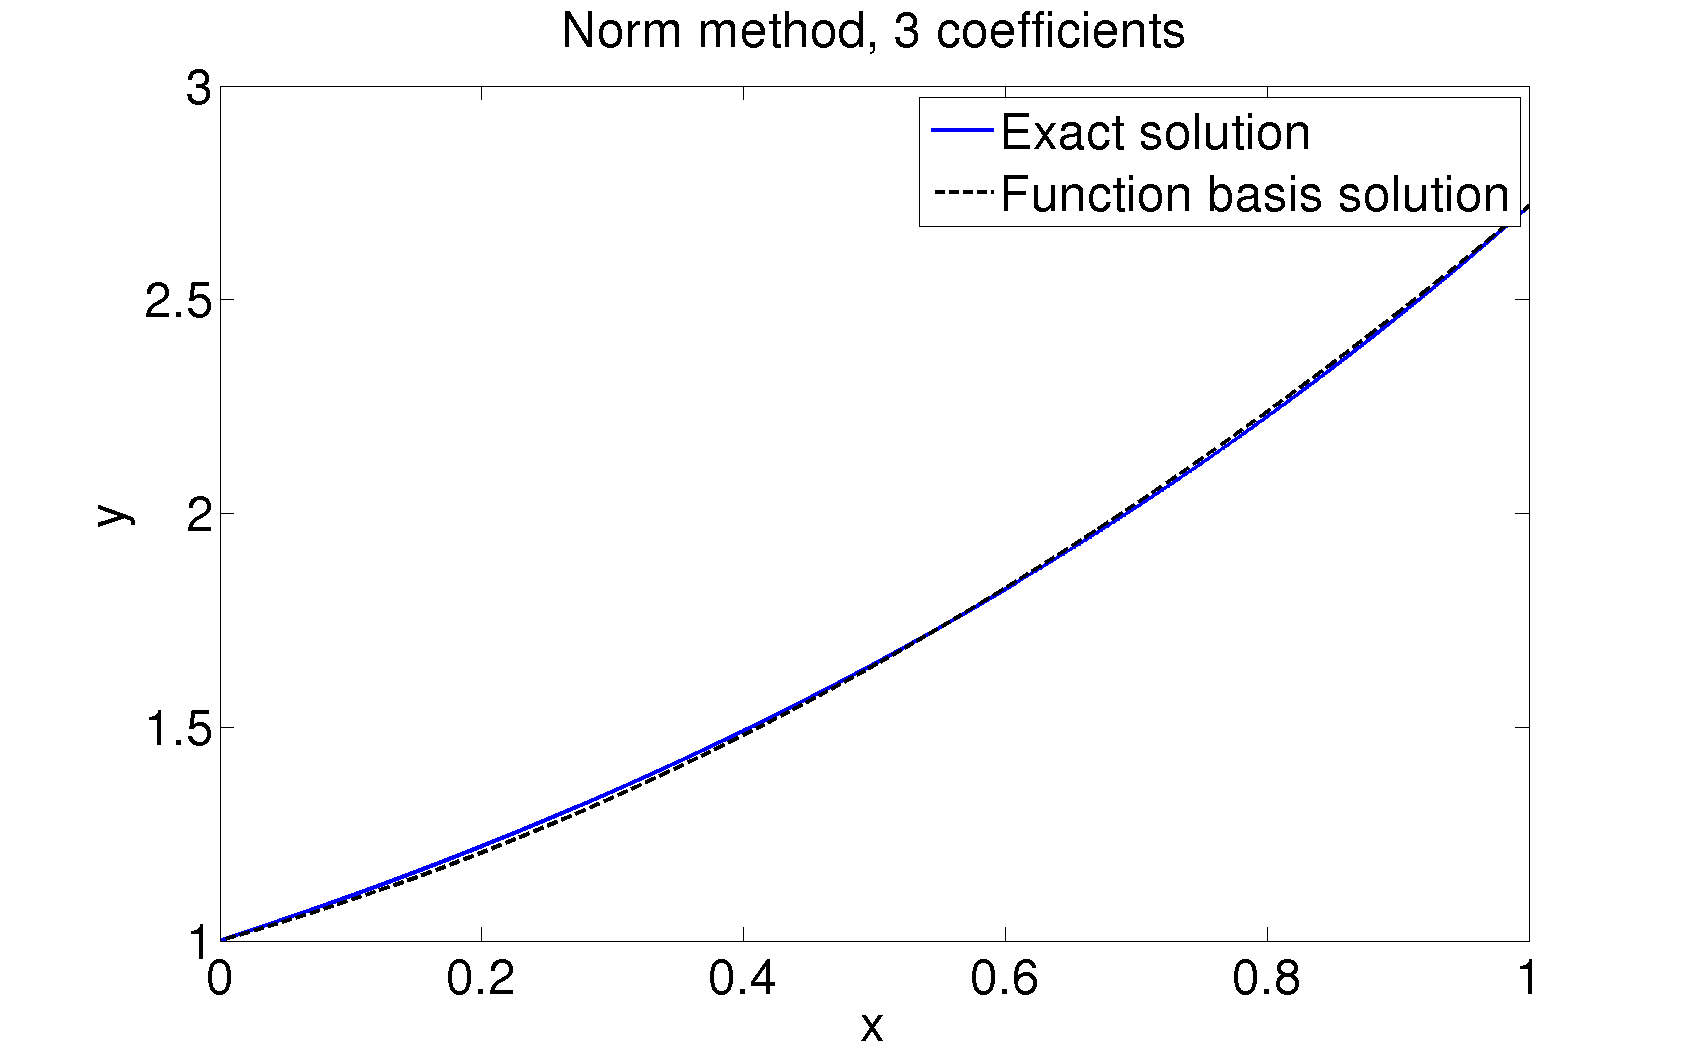
\includegraphics[width=\textwidth]{figures/Norm1}
      \end{center}
    \end{column}
  \end{columns}
\end{frame}


\subsection{Ritz methods}

\begin{frame}
  \frametitle{Ritz methods}

  General framework: working in Hilbert space $L_2$ define \emph{inner
    product}
  \begin{equation*}
    < u, v > = \int_a^b u \cdot v \, \text{d} x.
  \end{equation*} \pause
  Need ${\cal L}$ to be symmetric and positive definite.

  \vspace{1ex}

  Inner product can \emph{measure distance} on $L_2$: i.e., measure
  the distance to the ``exact solution'' of the ODE. \pause

  \vspace{1ex}

  So define \emph{energy} of the element $u$ as
  \begin{equation*}
    < {\cal L}(u), u > \,\, \ge 0,
  \end{equation*}
  where inequality follows by integration by parts. \pause Then to get
  solution minimize
  \begin{equation*}
    J(u) = < {\cal L}(u), u > - 2 < f, u >.
  \end{equation*}

\end{frame}

\begin{frame}
  \frametitle{Ritz method applied to a function basis}

  Can minimize the functional
  \begin{equation*}
    J(y) = < {\cal L}(y), y > - 2 < f, y >
  \end{equation*}
  when $y$ is given with respect to a function basis,
  \begin{equation*}
    y = \sum_j^n c_j u_j(x).
  \end{equation*} \pause

  Linearity means this is equivalent to minimizing quadratic form
  \begin{equation*}
    J(y) = \sum_{m,k}^n c_m c_k < {\cal L}(u_m), u_k > - 2 \sum_m c_m
    < f, u_m >.
  \end{equation*} \pause
  Know $u_j$, so re-express as a condition on $c_j$.

\end{frame}

\begin{frame}
  \frametitle{Ritz method applied to a function basis}

  \begin{equation*}
    y = \sum_j^n c_j u_j(x).
  \end{equation*}

  \begin{equation*}
    J(y) = \sum_{m,k}^n c_m c_k < {\cal L}(u_m), u_k > - 2 \sum_m c_m
    < f, u_m >.
  \end{equation*}

  Minimizing this functional requires
  \begin{align*}
    && \pda{}{c_m} J & = 0, & m = 1, \dots, n, \\
    \Rightarrow && \sum_m^n c_m < {\cal L}(u_m), u_k > & = < f, u_k >,
    & k = 1, \dots, n.
  \end{align*}
  This is just a linear system to solve.

\end{frame}

\begin{frame}
  \frametitle{Example}

  For the boundary value problem
  \begin{equation*}
    y'' = -\cos(x), \quad y(0) = 0 = y(\pi)
  \end{equation*}
  we have the exact solution $y(x) = \cos(x) + 2 x /\pi - 1$. \pause
  Symmetry of problem suggests the function basis
  \begin{equation*}
    u_j = \sin(2 j x):
  \end{equation*}
  satisfies boundary conditions and symmetry. \pause

  \vspace{1ex}

  We need to satisfy
  \begin{equation*}
    \sum_m^n c_m < {\cal L}(u_m), u_k >  = < f, u_k >.
  \end{equation*}
  Vector of unknowns $c_m$; known matrix has elements $A_{m,k} = <
  {\cal L}(u_m), u_k >$; known vector has elements $< f, u_k >$.

\end{frame}

\begin{frame}
  \frametitle{Example: 2}

  \begin{overlayarea}{\textwidth}{0.9\textheight}
    \only<1-2|handout:1>
    {

      The \emph{matrix} $A_{m,k} = < {\cal L}(u_m), u_k >$ has elements
      \begin{align*}
        < {\cal L}(u_m), u_k > & = -\int_0^{\pi} 4 m^2 \sin(2 m x)
        \sin(2 k
        x) \, \text{d} x \\
        & =
        \begin{cases}
          -2 \pi k^2, & \text{if $m = k$}, \\
          0, & \text{if $m \ne k$}
        \end{cases}.
      \end{align*}
    }
    \only<2|handout:1>
    {
      The \emph{vector} $< f, u_k >$ has elements
      \begin{align*}
        < f, u_k > & = \int_0^{\pi} -\cos(x) \sin(2 k x) \, \text{d} x \\
        & = \frac{4 k}{4 k^2 - 1}.
      \end{align*}
    }
    \only<3|handout:2>
    {
      \begin{align*}
        < {\cal L}(u_m), u_k > & = \begin{cases}
          -2 \pi k^2, & \text{if $m = k$}, \\
          0, & \text{if $m \ne k$}
        \end{cases}, \\
        < f, u_k > & = \frac{4 k}{4 k^2 - 1}.
      \end{align*}

      This gives a \emph{diagonal} system which can be solved to give
      \begin{equation*}
        c_m = \frac{2}{\pi m (4 m^2 - 1)}
      \end{equation*}
      and hence the approximation
      \begin{equation*}
        y = \frac{2}{\pi} \sum_{m=1}^n \frac{\sin(2 m x)}{m (4 m^2 - 1)}
      \end{equation*}
      which converges to the Fourier series in the limit $n \rightarrow
      \infty$.
    }
  \end{overlayarea}

\end{frame}

\begin{frame}
  \frametitle{Example: 3}

  \begin{columns}
    \begin{column}{0.4\textwidth}
      In fact even with very few coefficients the Ritz method is
      accurate. \pause

      \vspace{1ex}

      It also converges \pause quickly.
    \end{column}
    \begin{column}{0.6\textwidth}
      \begin{center}
        \includegraphics<1|handout:0>[width=\textwidth]{figures/Ritz1}
        \includegraphics<2|handout:0>[width=\textwidth]{figures/Ritz2}
        \includegraphics<3>[width=\textwidth]{figures/Ritz3}
      \end{center}
    \end{column}
  \end{columns}

\end{frame}

\section{Summary}

\subsection{Summary}

\begin{frame}
  \frametitle{Summary}

  \begin{itemize}
  \item When extreme accuracy is essential then function basis methods
    are often used.
  \item Collocation methods are popular; given the right choice of
    basis and collocation points the convergence can be faster than
    any polynomial, giving floating point accuracy with a few dozen
    basis functions at most.
  \item Norm and Ritz type methods do not use a grid at all; this can
    make them useful in complex domains, particular as a small part of
    a larger method (see finite elements).
  \item The complexity of these methods, particularly norm and Ritz,
    makes the work involved in setting up the problem quite
    extreme. The actual coding of the method is, however, very small
    for the impressive accuracy.
  \end{itemize}

\end{frame}

\end{document}



%%% Local Variables:
%%% mode: latex
%%% TeX-master: t
%%% End:
